% Chapter Template

\chapter{Long Short-Term Memory} % Main chapter title

\label{Chapter4} % Change X to a consecutive number; for referencing this chapter elsewhere, use \ref{ChapterX}

%----------------------------------------------------------------------------------------
%	SECTION 1
%----------------------------------------------------------------------------------------

\section{Understanding LSTMs}

Long Short Term Memory networks – usually just called \textit{LSTMs} – are a special kind of RNN, capable of learning long-term dependencies. They were introduced by Hochreiter and Schmidhuber (1997).

LSTMs are explicitly designed to avoid the long-term dependency problem. This allows the network to remember information for long periods of time.

All recurrent neural networks have the form of a chain of repeating modules of neural network. But the core of the LSTMs is the \textit{cell state}, that allows the network to keep a simple state information through the processing of all the time steps in the chain. An scheme of a LSTM architecture is described in figure \ref{fig:lstm}.

\begin{figure}
\begin{center}
  \makebox[\textwidth]{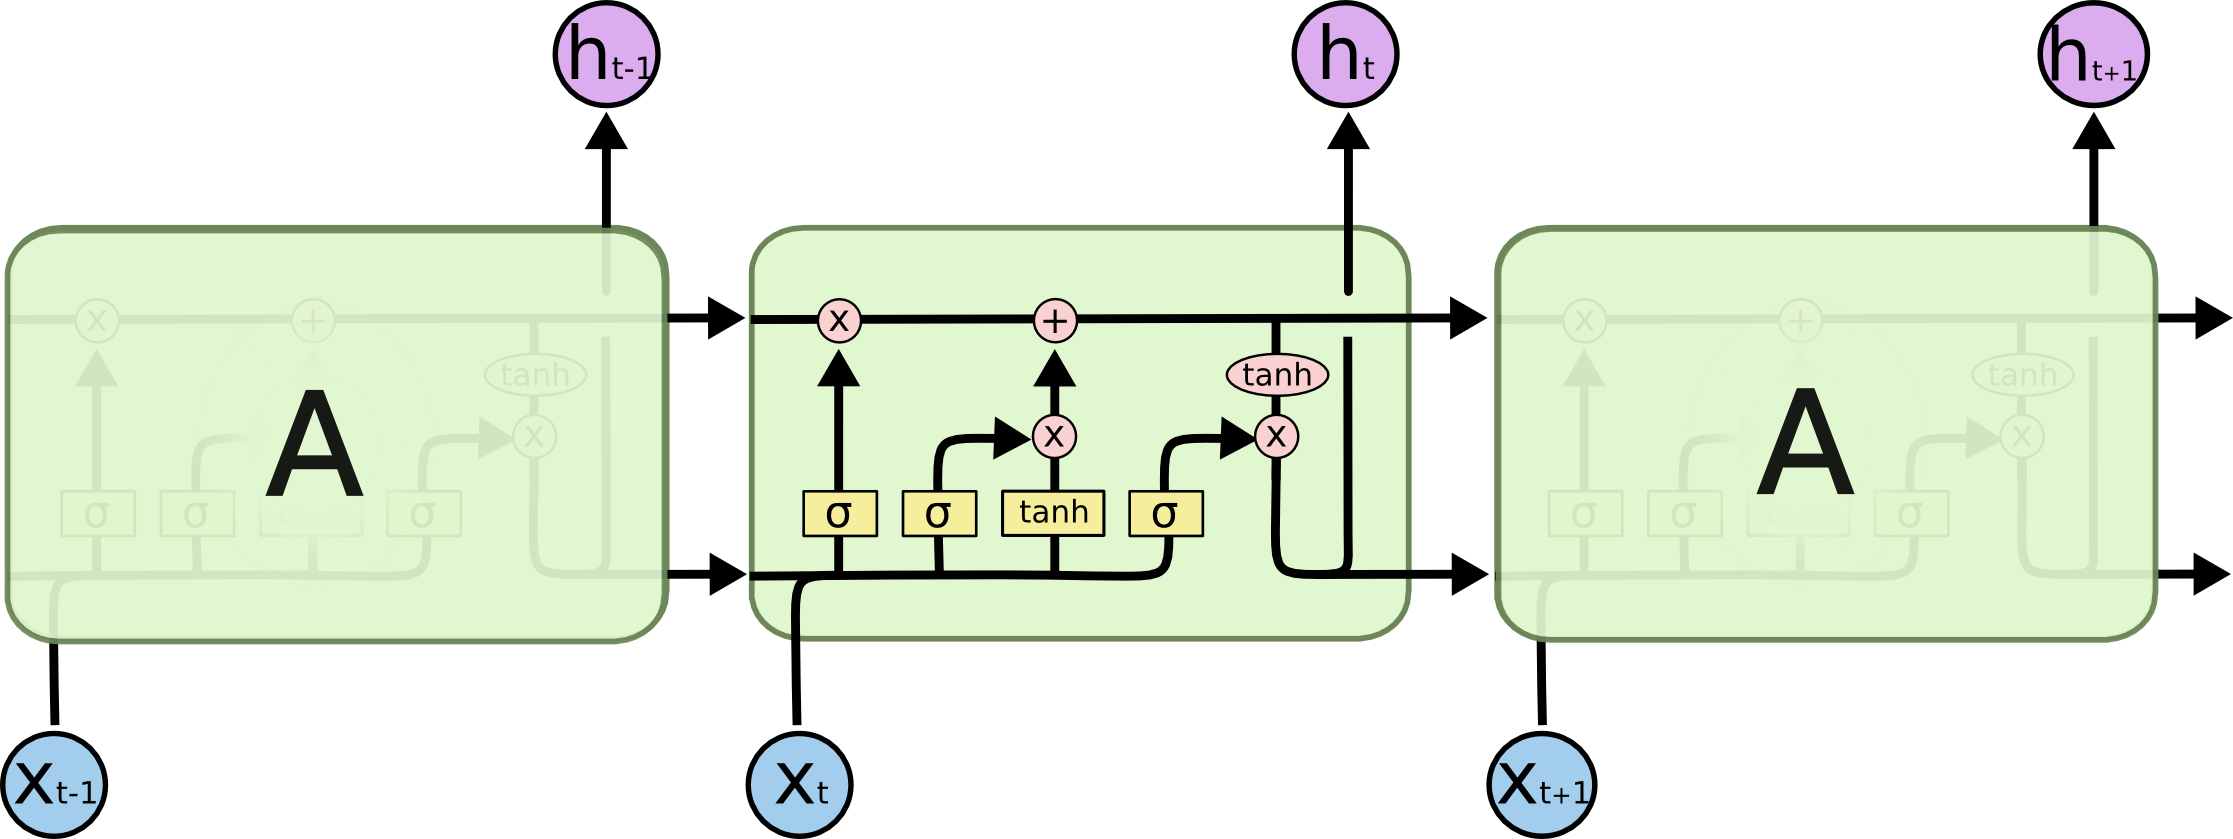
\includegraphics[width=\textwidth]{Figures/LSTM}}
\end{center}
\decoRule
\caption[LSTM architecture]{LSTM architecture.}
\label{fig:lstm}
\end{figure}

\section{Binary Classification}

The next sections describe the methodology applied to solve the binary classification problem using LSTMs

%-----------------------------------
%	SUBSECTION 1
%-----------------------------------
\subsection{Data Generation}

Before the ingestion of the data into the LSTM model, it has to be adapted to the architecture of the network.

Being \textit{samples} the total number of data, \textit{timesteps} the amount of rows to be ingested for each aircraft and \textit{features} the number of sensor data the input of the LSTM layer is defined by a tensor of shape:

\begin{verbatim}
    (samples, timesteps, features)
\end{verbatim}

The time steps used for the study will be 50, which means that for each aircraft batches of 50 time steps will be taken.
Using the \textit{zip} function over the data of the aircraft with id=1, which contains 192 cycles. The batches will be distributed this way:

\begin{verbatim}
    (0, 50)     -> from row 0 to row 50
    (1, 51)     -> from row 1 to row 51
    (2, 52)     -> from row 2 to row 52
    ...
    (111, 192)  -> from row 111 to row 192
\end{verbatim}

After the pre-processing, the input tensor will have the shape:

\begin{verbatim}
    (15631, 50, 25)
\end{verbatim}

To generate the labels, the values of the column \textit{label 1}, which was generated on the data preparation (see chapter \ref{Chapter3}), must be grouped by aircraft indicating if the engine failed within \textit{w1} cycles.

The result label tensor has the shape:

\begin{verbatim}
    (15631, 1)
\end{verbatim}

%-----------------------------------
%	SUBSECTION 2
%-----------------------------------

\subsection{Model definition}

As explained above, the architecture of the neural network is based on the use of LSTM layers. In this model two different LSTM layers are used to achieve better results.

To accomplish the binary classification, the output layer of the network is a Dense layer with a single output value. This value classifies between two different options: the aircraft will fail or not within the specified cycle.

To prevent over-fitting, two Dropout layers are concatenated after the output of both LSTM layers. This adds a regularization method that drops random units after the LSTM layers, avoiding the network to learn interdependent set of feature weights.

Finally, the loss function selected for this kind of classification problem is \textit{binary crossentropy} using \textit{Adam} as optimizer.

The diagram for the neural network is described in figure \ref{fig:binary-lstm-model}

\begin{figure}
\centering
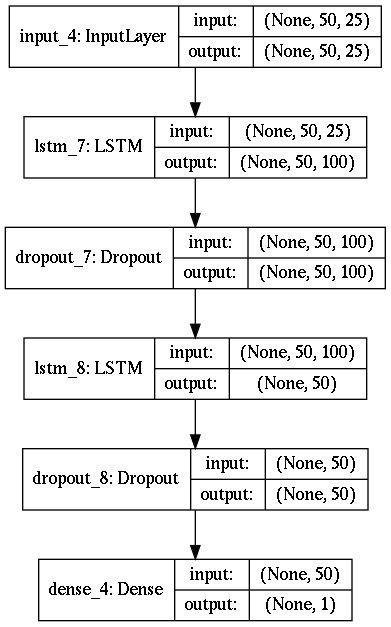
\includegraphics{Figures/binary-lstm-model}
\decoRule
\caption[Neural Network model for binary classification]{Neural Network model for binary classification.}
\label{fig:binary-lstm-model}
\end{figure}

\subsection{Training visualization}

Visualizing the output of the different layers of a network is one of the most useful tools to analyze the network performance. It could also help us to determine if the data analysis has been done correctly and allow us to see possible biases over the data distribution.

For the current network, the output of the last LSTM layer has been taken in account to do this analysis. The output of this layer is a tensor of size 50, which represents the hidden units of the LSTM. To extract the information contain by those celds, the \textit{Principal Component Analysis} (PCA) function has been chosen.

PCA is a mathematical function that allows us to summarize huge features sets. For this dissertation, two principal components has been configured. In figure \ref{fig:binary-lstm-pca} you can see a graphical representation of this components.

In this figure we can clearly see how the values conforms to main clusters of data. This has a lot of sense since we are trying to classify the data in two different groups.

\begin{figure}
\centering
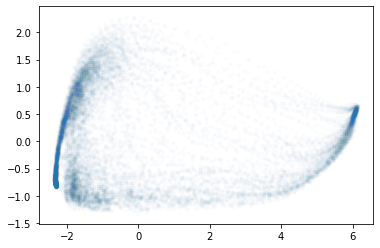
\includegraphics{Figures/lstm-visualization}
\decoRule
\caption[PCA applied over LSTM output]{PCA applied over LSTM output.}
\label{fig:binary-lstm-pca}
\end{figure}


\subsection{Results and model evaluation}

After the model is trained using batches of data of size 200. The validation split selected for the data is 5\%.

The evolution of the loss and accuracy during the model training can be seen in the figures \ref{fig:binary-lstm-loss} and \ref{fig:binary-lstm-acc}

The final accuracy obtained is 98\% so we can conclude that the network works very well for this task. To evaluate the results against the ground truth data a comparison graph has been generated. This graph can be seen in figure \ref{fig:binary-lstm-results}.

\begin{figure}
\begin{center}
  \makebox[\textwidth]{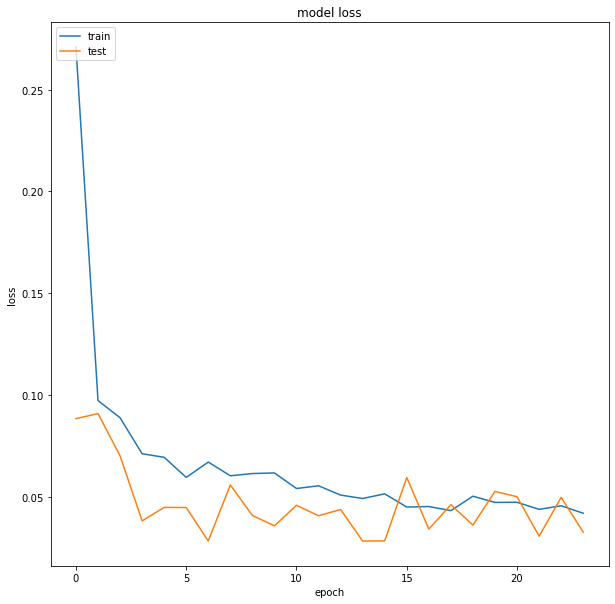
\includegraphics[width=\textwidth]{Figures/binary-lstm-loss}}
\end{center}
\decoRule
\caption[Binary Classification Model Loss]{Binary Classification Model Loss.}
\label{fig:binary-lstm-loss}\end{figure}

\begin{figure}
\begin{center}
  \makebox[\textwidth]{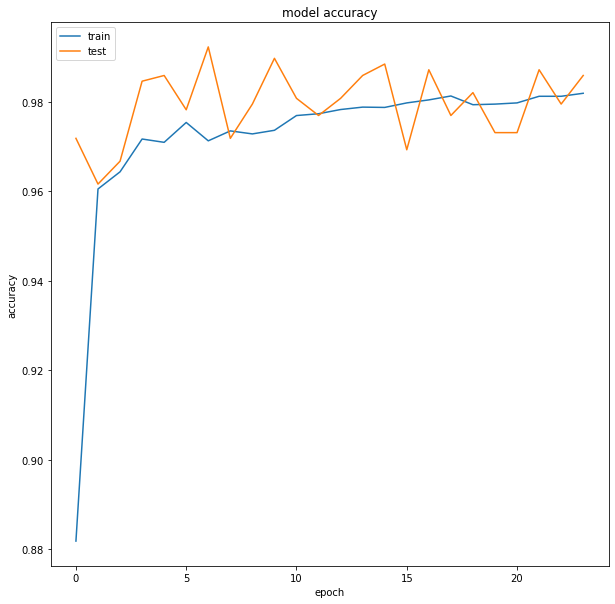
\includegraphics[width=\textwidth]{Figures/binary-lstm-acc}}
\end{center}
\decoRule
\caption[Binary Classification Model Accuracy]{Binary Classification Model Accuracy.}
\label{fig:binary-lstm-acc}
\end{figure}

\begin{figure}
\begin{center}
  \makebox[\textwidth]{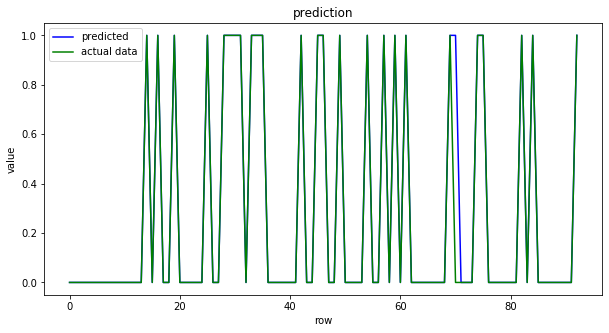
\includegraphics[width=\textwidth]{Figures/binary-lstm-results}}
\end{center}
\decoRule
\caption[Result comparison between Binary LSTM Model and Ground Truth data]{Result comparison between Binary LSTM Model and Ground Truth data.}
\label{fig:binary-lstm-results}
\end{figure}


\section{Regression Model}

The next sections describe the methodology applied to solve the regression problem using LSTMs


\subsection{Data Generation}

Before the ingestion of the data into the LSTM model, it has to be adapted to the architecture of the network.

Being \textit{samples} the total number of data, \textit{timesteps} the amount of rows to be ingested for each aircraft and \textit{features} the number of sensor data the input of the LSTM layer is defined by a tensor of shape:

\begin{verbatim}
    (samples, timesteps, features)
\end{verbatim}

The time steps used for the study will be 50, which means that for each aircraft batches of 50 time steps will be taken.
Using the \textit{zip} function over the data of the aircraft with id=1, which contains 192 cycles. The batches will be distributed this way:

\begin{verbatim}
    (0, 50)     -> from row 0 to row 50
    (1, 51)     -> from row 1 to row 51
    (2, 52)     -> from row 2 to row 52
    ...
    (111, 192)  -> from row 111 to row 192
\end{verbatim}

After the pre-processing, the input tensor will have the shape:

\begin{verbatim}
    (15631, 50, 25)
\end{verbatim}

For this type of regression model the labels are the values of the column \textit{RUL}, which was generated on the data preparation (see chapter \ref{Chapter3}).

The result label tensor has the shape:

\begin{verbatim}
    (15631, 1)
\end{verbatim}


\subsection{Model definition}

As explained above, the architecture of the neural network is based on the use of LSTM layers. In this model two different LSTM layers are used to achieve better results.

To accomplish the binary classification, the output layer of the network is a Dense layer with a single output value. This linear value is generated by the network output and represents the \textit{RUL} that the network calculates for an especific aircraft. Finally, an linear activation function is added to the last layer.

To prevent over-fitting, two Dropout layers are concatenated after the output of both LSTM layers. This adds a regularization method that drops random units after the LSTM layers, avoiding the network to learn interdependent set of feature weights.

The loss function selected for this kind of classification problem is \textit{binary crossentropy} using \textit{RMSProp} as optimizer.

For the regression model the metric used is \textit{MAE}, also, in this dissertation the \textit{Coefficient of Determination} (R squared) metric function has been implemented.

The diagram for the neural network is described in figure \ref{fig:regression-lstm-model}

\begin{figure}
\centering
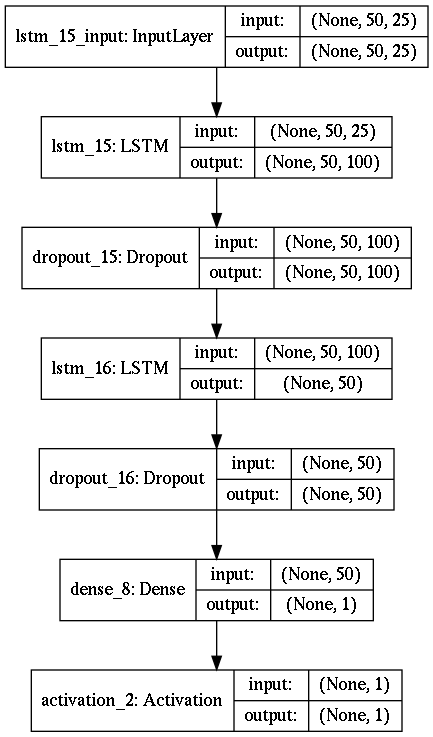
\includegraphics{Figures/regression-lstm-model}
\decoRule
\caption[Neural Network for regression model]{Neural Network for regression model.}
\label{fig:regression-lstm-model}
\end{figure}

\subsection{Results and model evaluation}

After the model is trained using batches of data of size 200. The validation split selected for the data is 5\%.

The evolution of the loss and metrics during the model training can be seen in the figures \ref{fig:regression-lstm-loss}, \ref{fig:regression-lstm-r2} and \ref{fig:regression-lstm-mae}

The final results obtained for \textit{MAE} and \textit{R-square} are 11.93 and 0.81 respectively.To evaluate the results against the ground truth data a comparison graph has been generated. This graph can be seen in figure \ref{fig:regression-lstm-results}.

\begin{figure}
\begin{center}
  \makebox[\textwidth]{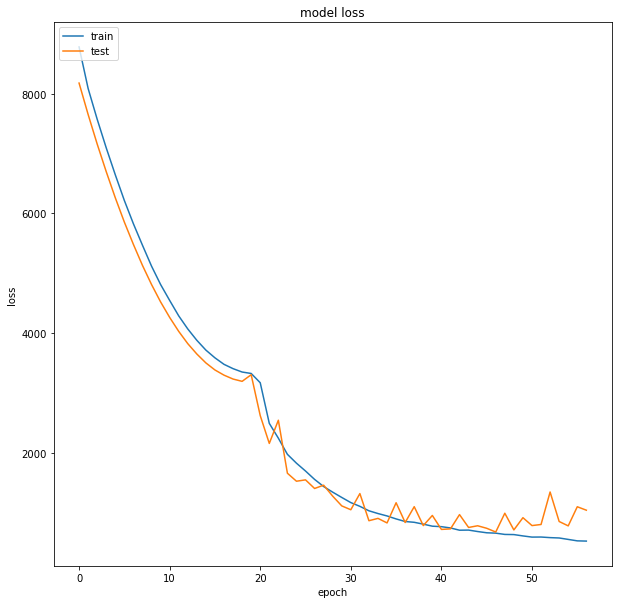
\includegraphics[width=\textwidth]{Figures/regression-lstm-loss}}
\end{center}
\decoRule
\caption[Regression Model Loss]{Regression Model Loss.}
\label{fig:regression-lstm-loss}\end{figure}

\begin{figure}
\begin{center}
  \makebox[\textwidth]{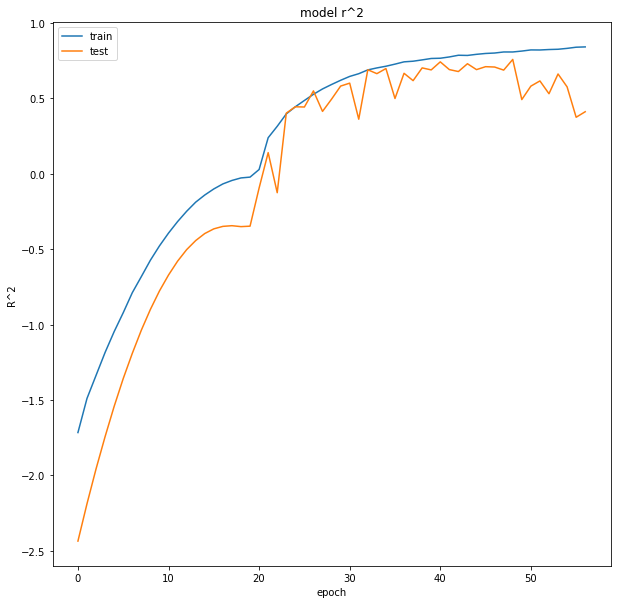
\includegraphics[width=\textwidth]{Figures/regression-lstm-r2}}
\end{center}
\decoRule
\caption[R2 model]{R2 model.}
\label{fig:regression-lstm-r2}
\end{figure}

\begin{figure}
\begin{center}
  \makebox[\textwidth]{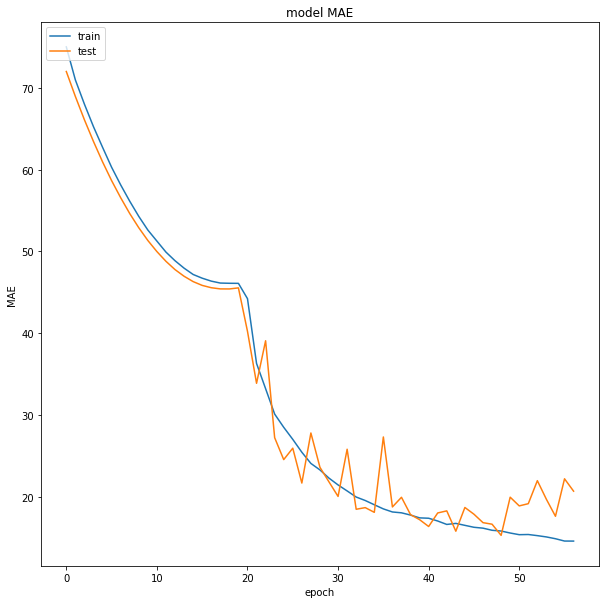
\includegraphics[width=\textwidth]{Figures/regression-lstm-mae}}
\end{center}
\decoRule
\caption[MAE model]{MAE model.}
\label{fig:regression-lstm-mae}
\end{figure}

\begin{figure}
\begin{center}
  \makebox[\textwidth]{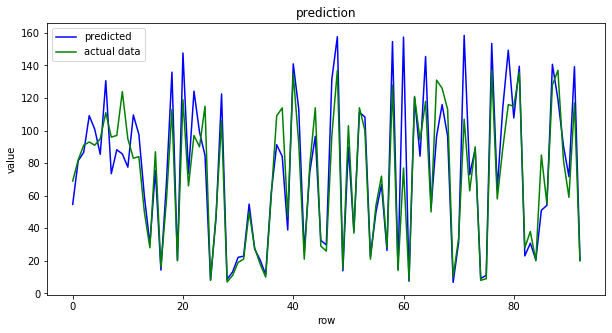
\includegraphics[width=\textwidth]{Figures/regression-lstm-results}}
\end{center}
\decoRule
\caption[Result comparison between Regression LSTM Model and Ground Truth data]{Result comparison between Regression LSTM Model and Ground Truth data.}
\label{fig:regression-lstm-results}
\end{figure}
